\documentclass[11pt,]{article}
\usepackage{lmodern}
\usepackage{amssymb,amsmath}
\usepackage{ifxetex,ifluatex}
\usepackage{fixltx2e} % provides \textsubscript
\ifnum 0\ifxetex 1\fi\ifluatex 1\fi=0 % if pdftex
  \usepackage[T1]{fontenc}
  \usepackage[utf8]{inputenc}
\else % if luatex or xelatex
  \ifxetex
    \usepackage{mathspec}
  \else
    \usepackage{fontspec}
  \fi
  \defaultfontfeatures{Ligatures=TeX,Scale=MatchLowercase}
\fi
% use upquote if available, for straight quotes in verbatim environments
\IfFileExists{upquote.sty}{\usepackage{upquote}}{}
% use microtype if available
\IfFileExists{microtype.sty}{%
\usepackage{microtype}
\UseMicrotypeSet[protrusion]{basicmath} % disable protrusion for tt fonts
}{}
\usepackage[margin=1in]{geometry}
\usepackage{hyperref}
\hypersetup{unicode=true,
            pdftitle={Package vars},
            pdfauthor={Paul GUILLOTTE \& Jules CORBEL},
            pdfborder={0 0 0},
            breaklinks=true}
\urlstyle{same}  % don't use monospace font for urls
\usepackage{color}
\usepackage{fancyvrb}
\newcommand{\VerbBar}{|}
\newcommand{\VERB}{\Verb[commandchars=\\\{\}]}
\DefineVerbatimEnvironment{Highlighting}{Verbatim}{commandchars=\\\{\}}
% Add ',fontsize=\small' for more characters per line
\usepackage{framed}
\definecolor{shadecolor}{RGB}{248,248,248}
\newenvironment{Shaded}{\begin{snugshade}}{\end{snugshade}}
\newcommand{\KeywordTok}[1]{\textcolor[rgb]{0.13,0.29,0.53}{\textbf{{#1}}}}
\newcommand{\DataTypeTok}[1]{\textcolor[rgb]{0.13,0.29,0.53}{{#1}}}
\newcommand{\DecValTok}[1]{\textcolor[rgb]{0.00,0.00,0.81}{{#1}}}
\newcommand{\BaseNTok}[1]{\textcolor[rgb]{0.00,0.00,0.81}{{#1}}}
\newcommand{\FloatTok}[1]{\textcolor[rgb]{0.00,0.00,0.81}{{#1}}}
\newcommand{\ConstantTok}[1]{\textcolor[rgb]{0.00,0.00,0.00}{{#1}}}
\newcommand{\CharTok}[1]{\textcolor[rgb]{0.31,0.60,0.02}{{#1}}}
\newcommand{\SpecialCharTok}[1]{\textcolor[rgb]{0.00,0.00,0.00}{{#1}}}
\newcommand{\StringTok}[1]{\textcolor[rgb]{0.31,0.60,0.02}{{#1}}}
\newcommand{\VerbatimStringTok}[1]{\textcolor[rgb]{0.31,0.60,0.02}{{#1}}}
\newcommand{\SpecialStringTok}[1]{\textcolor[rgb]{0.31,0.60,0.02}{{#1}}}
\newcommand{\ImportTok}[1]{{#1}}
\newcommand{\CommentTok}[1]{\textcolor[rgb]{0.56,0.35,0.01}{\textit{{#1}}}}
\newcommand{\DocumentationTok}[1]{\textcolor[rgb]{0.56,0.35,0.01}{\textbf{\textit{{#1}}}}}
\newcommand{\AnnotationTok}[1]{\textcolor[rgb]{0.56,0.35,0.01}{\textbf{\textit{{#1}}}}}
\newcommand{\CommentVarTok}[1]{\textcolor[rgb]{0.56,0.35,0.01}{\textbf{\textit{{#1}}}}}
\newcommand{\OtherTok}[1]{\textcolor[rgb]{0.56,0.35,0.01}{{#1}}}
\newcommand{\FunctionTok}[1]{\textcolor[rgb]{0.00,0.00,0.00}{{#1}}}
\newcommand{\VariableTok}[1]{\textcolor[rgb]{0.00,0.00,0.00}{{#1}}}
\newcommand{\ControlFlowTok}[1]{\textcolor[rgb]{0.13,0.29,0.53}{\textbf{{#1}}}}
\newcommand{\OperatorTok}[1]{\textcolor[rgb]{0.81,0.36,0.00}{\textbf{{#1}}}}
\newcommand{\BuiltInTok}[1]{{#1}}
\newcommand{\ExtensionTok}[1]{{#1}}
\newcommand{\PreprocessorTok}[1]{\textcolor[rgb]{0.56,0.35,0.01}{\textit{{#1}}}}
\newcommand{\AttributeTok}[1]{\textcolor[rgb]{0.77,0.63,0.00}{{#1}}}
\newcommand{\RegionMarkerTok}[1]{{#1}}
\newcommand{\InformationTok}[1]{\textcolor[rgb]{0.56,0.35,0.01}{\textbf{\textit{{#1}}}}}
\newcommand{\WarningTok}[1]{\textcolor[rgb]{0.56,0.35,0.01}{\textbf{\textit{{#1}}}}}
\newcommand{\AlertTok}[1]{\textcolor[rgb]{0.94,0.16,0.16}{{#1}}}
\newcommand{\ErrorTok}[1]{\textcolor[rgb]{0.64,0.00,0.00}{\textbf{{#1}}}}
\newcommand{\NormalTok}[1]{{#1}}
\usepackage{graphicx,grffile}
\makeatletter
\def\maxwidth{\ifdim\Gin@nat@width>\linewidth\linewidth\else\Gin@nat@width\fi}
\def\maxheight{\ifdim\Gin@nat@height>\textheight\textheight\else\Gin@nat@height\fi}
\makeatother
% Scale images if necessary, so that they will not overflow the page
% margins by default, and it is still possible to overwrite the defaults
% using explicit options in \includegraphics[width, height, ...]{}
\setkeys{Gin}{width=\maxwidth,height=\maxheight,keepaspectratio}
\IfFileExists{parskip.sty}{%
\usepackage{parskip}
}{% else
\setlength{\parindent}{0pt}
\setlength{\parskip}{6pt plus 2pt minus 1pt}
}
\setlength{\emergencystretch}{3em}  % prevent overfull lines
\providecommand{\tightlist}{%
  \setlength{\itemsep}{0pt}\setlength{\parskip}{0pt}}
\setcounter{secnumdepth}{5}
% Redefines (sub)paragraphs to behave more like sections
\ifx\paragraph\undefined\else
\let\oldparagraph\paragraph
\renewcommand{\paragraph}[1]{\oldparagraph{#1}\mbox{}}
\fi
\ifx\subparagraph\undefined\else
\let\oldsubparagraph\subparagraph
\renewcommand{\subparagraph}[1]{\oldsubparagraph{#1}\mbox{}}
\fi

%%% Use protect on footnotes to avoid problems with footnotes in titles
\let\rmarkdownfootnote\footnote%
\def\footnote{\protect\rmarkdownfootnote}

%%% Change title format to be more compact
\usepackage{titling}

% Create subtitle command for use in maketitle
\newcommand{\subtitle}[1]{
  \posttitle{
    \begin{center}\large#1\end{center}
    }
}

\setlength{\droptitle}{-2em}

  \title{Package vars}
    \pretitle{\vspace{\droptitle}\centering\huge}
  \posttitle{\par}
    \author{Paul GUILLOTTE \& Jules CORBEL}
    \preauthor{\centering\large\emph}
  \postauthor{\par}
      \predate{\centering\large\emph}
  \postdate{\par}
    \date{01/02/2019}


\begin{document}
\maketitle
\begin{abstract}
bbbbb
\end{abstract}

{
\setcounter{tocdepth}{2}
\tableofcontents
}
\section*{Introduction}\label{introduction}
\addcontentsline{toc}{section}{Introduction}

\section{Visualisation des séries}\label{visualisation-des-series}

Nous nous intéressons dans cette partie aux différentes séries
trimestrielles à notre disposition. Dans un premier temps, nous nous
intéressons aux corrélations entre les variables deux à deux afin de
nous faire une première idée du lien qu'il existe entre les variables.

\subsection{Masse salariale}\label{masse-salariale}

\begin{Shaded}
\begin{Highlighting}[]
  \NormalTok{MSE <-}\StringTok{ }\KeywordTok{ts}\NormalTok{(trim$MSE, }\DataTypeTok{start =} \DecValTok{1990}\NormalTok{, }\DataTypeTok{end =} \KeywordTok{c}\NormalTok{(}\DecValTok{2017}\NormalTok{, }\DecValTok{2}\NormalTok{), }\DataTypeTok{frequency=}\DecValTok{4}\NormalTok{)}
  \KeywordTok{plot}\NormalTok{(MSE, }\DataTypeTok{main=}\StringTok{"Evolution trimestrielle de la masse salariale"}\NormalTok{, }\DataTypeTok{xaxt=}\StringTok{"n"}\NormalTok{, }\DataTypeTok{cex.main=}\FloatTok{0.9}\NormalTok{)}
  \KeywordTok{axis}\NormalTok{(}\DataTypeTok{side=}\DecValTok{1}\NormalTok{, }\DataTypeTok{at=}\KeywordTok{seq}\NormalTok{(}\DecValTok{1990}\NormalTok{,}\DecValTok{2015}\NormalTok{,}\DecValTok{5}\NormalTok{), }\DataTypeTok{labels=}\KeywordTok{c}\NormalTok{(}\StringTok{"1990Q1"}\NormalTok{, }\StringTok{"1995Q1"}\NormalTok{, }\StringTok{"2000Q1"}\NormalTok{, }\StringTok{"2005Q1"}\NormalTok{, }
                                             \StringTok{"2010Q1"}\NormalTok{, }\StringTok{"2015Q1"}\NormalTok{))}
\end{Highlighting}
\end{Shaded}

\begin{center}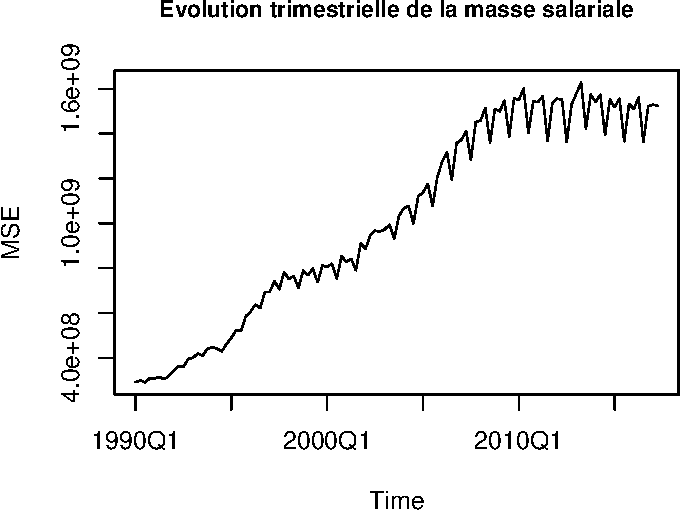
\includegraphics{doc_files/figure-latex/unnamed-chunk-1-1} \end{center}

\begin{Shaded}
\begin{Highlighting}[]
  \KeywordTok{par}\NormalTok{(}\DataTypeTok{mfrow=}\KeywordTok{c}\NormalTok{(}\DecValTok{1}\NormalTok{,}\DecValTok{2}\NormalTok{), }\DataTypeTok{cex.main=}\FloatTok{0.8}\NormalTok{)}
  \KeywordTok{acf}\NormalTok{(MSE, }\DataTypeTok{main=}\StringTok{"Auto-corrélation de la}
\StringTok{      masse salariale trimestrielle"}\NormalTok{, }\DataTypeTok{lag.max=}\DecValTok{20}\NormalTok{)}
  \KeywordTok{pacf}\NormalTok{(MSE, }\DataTypeTok{main=}\StringTok{"Autocorrélation partielle}
\StringTok{       de la masse salariale trimestrielle"}\NormalTok{, }\DataTypeTok{lag.max=}\DecValTok{20}\NormalTok{)}
\end{Highlighting}
\end{Shaded}

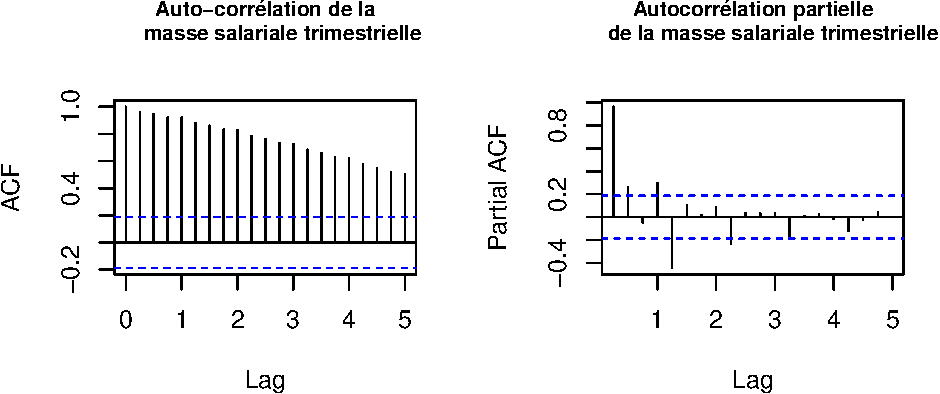
\includegraphics{doc_files/figure-latex/unnamed-chunk-2-1.pdf}

\begin{Shaded}
\begin{Highlighting}[]
  \KeywordTok{kpss.test}\NormalTok{(MSE)}
\end{Highlighting}
\end{Shaded}

\begin{verbatim}
## Warning in kpss.test(MSE): p-value smaller than printed p-value
\end{verbatim}

\begin{verbatim}
## 
##  KPSS Test for Level Stationarity
## 
## data:  MSE
## KPSS Level = 3.6772, Truncation lag parameter = 2, p-value = 0.01
\end{verbatim}

La masse salariale trimestrielle possède une composante de tendance de
1990 à 2010. La série tend par la suite à stagner. Nous remarquons
également une saisonnalité sur cette série, qui est de plus en plus
marquée à mesure que le temps passe.

Comme la série comporte une tendance et une saisonnalité, elle ne
correspond pas aux deux premières conditions de la stationnarité du
second ordre, soit que la série possède une moyenne et un écart-type
constants. Cela est confirmé par la fonction ACF qui décroît
régulièrement. Nous effectuons également un test de KPSS servant à
vérifier si la série est stationnaire ou non (sous l'hypothèse \(H_{0}\)
la série est stationnaire, et sous l'hypothèse \(H_{1}\) elle ne l'est
pas \textbf{Préciser plus clairement à quoi correspond la stationnarité
dans ce test + Ajouter d'autres tests de stationnarité}). La p-value est
de 0.01 ce qui nous confirme que la série n'est pas stationnaire avec un
risque de première espèce de 5\%.

\subsection{PIB}\label{pib}

\begin{Shaded}
\begin{Highlighting}[]
  \NormalTok{PIB <-}\StringTok{ }\KeywordTok{ts}\NormalTok{(trim$PIB, }\DataTypeTok{start =} \DecValTok{1990}\NormalTok{, }\DataTypeTok{end =} \KeywordTok{c}\NormalTok{(}\DecValTok{2017}\NormalTok{, }\DecValTok{1}\NormalTok{), }\DataTypeTok{frequency=}\DecValTok{4}\NormalTok{)}
  \KeywordTok{plot}\NormalTok{(PIB, }\DataTypeTok{main=}\StringTok{"Evolution trimestrielle du PIB"}\NormalTok{,}\DataTypeTok{xaxt=}\StringTok{"n"}\NormalTok{)}
  \KeywordTok{axis}\NormalTok{(}\DataTypeTok{side=}\DecValTok{1}\NormalTok{, }\DataTypeTok{at=}\KeywordTok{seq}\NormalTok{(}\DecValTok{1990}\NormalTok{,}\DecValTok{2015}\NormalTok{,}\DecValTok{5}\NormalTok{), }\DataTypeTok{labels=}\KeywordTok{c}\NormalTok{(}\StringTok{"1990Q1"}\NormalTok{, }\StringTok{"1995Q1"}\NormalTok{, }\StringTok{"2000Q1"}\NormalTok{, }\StringTok{"2005Q1"}\NormalTok{, }\StringTok{"2010Q1"}\NormalTok{, }\StringTok{"2015Q1"}\NormalTok{))}
\end{Highlighting}
\end{Shaded}

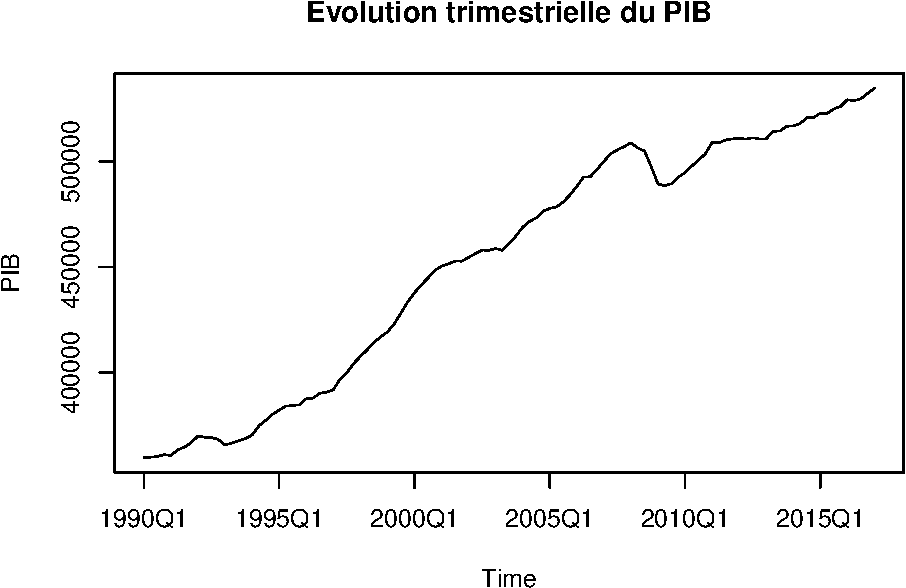
\includegraphics{doc_files/figure-latex/unnamed-chunk-3-1.pdf}

\begin{Shaded}
\begin{Highlighting}[]
  \KeywordTok{par}\NormalTok{(}\DataTypeTok{mfrow=}\KeywordTok{c}\NormalTok{(}\DecValTok{1}\NormalTok{,}\DecValTok{2}\NormalTok{))}
  \KeywordTok{acf}\NormalTok{(PIB, }\DataTypeTok{main=}\StringTok{"Auto-corrélation }
\StringTok{      du PIB trimestriel"}\NormalTok{, }\DataTypeTok{lag.max=}\DecValTok{20}\NormalTok{)}
  \KeywordTok{pacf}\NormalTok{(PIB, }\DataTypeTok{main=}\StringTok{"Autocorrélation partielle}
\StringTok{       du PIB trimestriel"}\NormalTok{, }\DataTypeTok{lag.max=}\DecValTok{20}\NormalTok{)}
\end{Highlighting}
\end{Shaded}

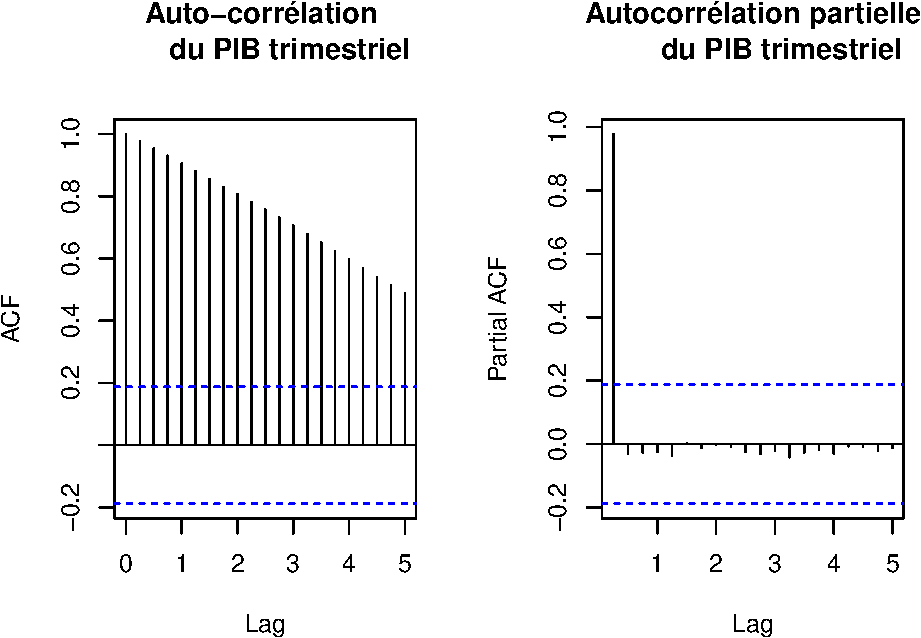
\includegraphics{doc_files/figure-latex/unnamed-chunk-3-2.pdf}

\begin{Shaded}
\begin{Highlighting}[]
  \KeywordTok{par}\NormalTok{(}\DataTypeTok{mfrow=}\KeywordTok{c}\NormalTok{(}\DecValTok{1}\NormalTok{,}\DecValTok{1}\NormalTok{))}
  \KeywordTok{kpss.test}\NormalTok{(PIB)}
\end{Highlighting}
\end{Shaded}

\begin{verbatim}
## Warning in kpss.test(PIB): p-value smaller than printed p-value
\end{verbatim}

\begin{verbatim}
## 
##  KPSS Test for Level Stationarity
## 
## data:  PIB
## KPSS Level = 3.6473, Truncation lag parameter = 2, p-value = 0.01
\end{verbatim}

Comme pour la masse salariale, le PIB annuel possède une tendance.
Cependant, il ne semble pas posséder de saisonnalité. Cette série n'est
donc pas non plus stationnaire. Nous effectuons à nouveau un test de
KPSS. La p-value est de 0.01 ce qui nous confirme que la série n'est pas
stationnaire avec un risque de première espèce de 5\%.

\subsection{SMIC}\label{smic}

\begin{Shaded}
\begin{Highlighting}[]
  \NormalTok{SMIC <-}\StringTok{ }\KeywordTok{ts}\NormalTok{(trim$SMIC, }\DataTypeTok{start =} \KeywordTok{c}\NormalTok{(}\DecValTok{1990}\NormalTok{,}\DecValTok{1}\NormalTok{), }\DataTypeTok{end =} \KeywordTok{c}\NormalTok{(}\DecValTok{2017}\NormalTok{, }\DecValTok{4}\NormalTok{), }\DataTypeTok{frequency =} \DecValTok{4}\NormalTok{)}
  \KeywordTok{plot}\NormalTok{(SMIC, }\DataTypeTok{main=}\StringTok{"Evolution trimestrielle du SMIC"}\NormalTok{, }\DataTypeTok{xaxt=}\StringTok{"n"}\NormalTok{)}
  \KeywordTok{axis}\NormalTok{(}\DataTypeTok{side=}\DecValTok{1}\NormalTok{, }\DataTypeTok{at=}\KeywordTok{seq}\NormalTok{(}\DecValTok{1990}\NormalTok{,}\DecValTok{2015}\NormalTok{,}\DecValTok{5}\NormalTok{), }\DataTypeTok{labels=}\KeywordTok{c}\NormalTok{(}\StringTok{"1990Q1"}\NormalTok{, }\StringTok{"1995Q1"}\NormalTok{, }\StringTok{"2000Q1"}\NormalTok{, }\StringTok{"2005Q1"}\NormalTok{, }\StringTok{"2010Q1"}\NormalTok{, }\StringTok{"2015Q1"}\NormalTok{))}
\end{Highlighting}
\end{Shaded}

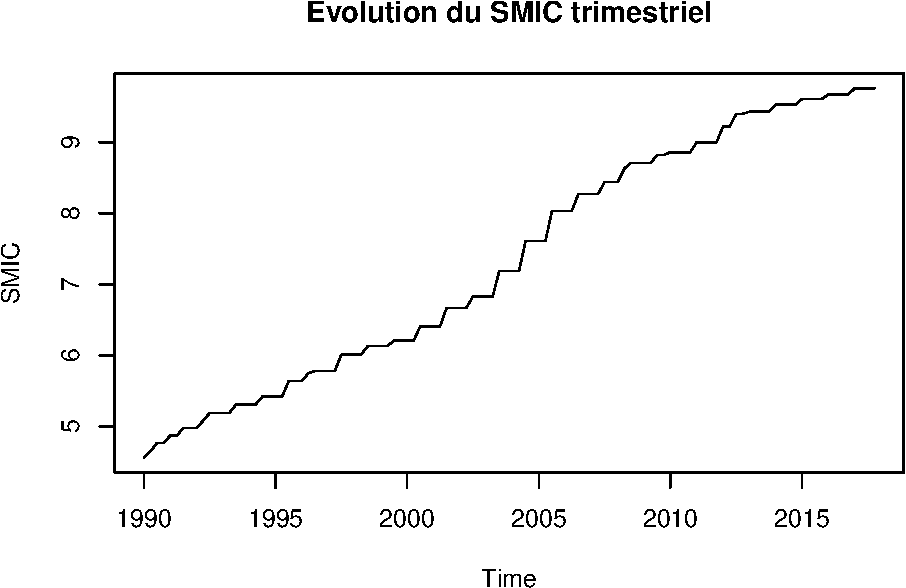
\includegraphics{doc_files/figure-latex/unnamed-chunk-4-1.pdf}

\begin{Shaded}
\begin{Highlighting}[]
  \KeywordTok{par}\NormalTok{(}\DataTypeTok{mfrow=}\KeywordTok{c}\NormalTok{(}\DecValTok{1}\NormalTok{,}\DecValTok{2}\NormalTok{))}
  \KeywordTok{acf}\NormalTok{(SMIC, }\DataTypeTok{main=}\StringTok{"Auto-corrélation du}
\StringTok{      SMIC trimestriel"}\NormalTok{, }\DataTypeTok{lag.max=}\DecValTok{20}\NormalTok{)}
  \KeywordTok{pacf}\NormalTok{(SMIC, }\DataTypeTok{main=}\StringTok{"Autocorrélation partielle}
\StringTok{       du SMIC trimestriel"}\NormalTok{, }\DataTypeTok{lag.max=}\DecValTok{20}\NormalTok{)}
\end{Highlighting}
\end{Shaded}

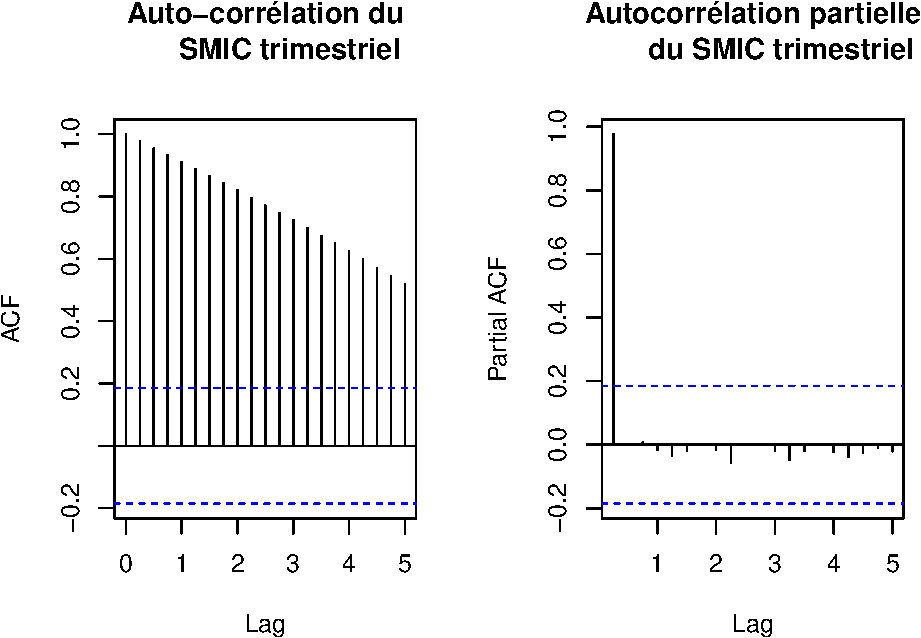
\includegraphics{doc_files/figure-latex/unnamed-chunk-4-2.pdf}

\begin{Shaded}
\begin{Highlighting}[]
  \KeywordTok{par}\NormalTok{(}\DataTypeTok{mfrow=}\KeywordTok{c}\NormalTok{(}\DecValTok{1}\NormalTok{,}\DecValTok{1}\NormalTok{))}
  \KeywordTok{kpss.test}\NormalTok{(SMIC)}
\end{Highlighting}
\end{Shaded}

\begin{verbatim}
## Warning in kpss.test(SMIC): p-value smaller than printed p-value
\end{verbatim}

\begin{verbatim}
## 
##  KPSS Test for Level Stationarity
## 
## data:  SMIC
## KPSS Level = 3.8382, Truncation lag parameter = 2, p-value = 0.01
\end{verbatim}

Au regard de la représentation graphique, on s'aperçoit qu'il y a bien
une tendance. Pour la saisonnalité, il est plus difficile de savoir s'il
en existe une ou pas, puisque la série semble augmenter seulement à
certains temps.

\subsection{Taux de chômage des
femmes}\label{taux-de-chomage-des-femmes}

\begin{Shaded}
\begin{Highlighting}[]
  \NormalTok{TCHOF <-}\StringTok{ }\KeywordTok{ts}\NormalTok{(trim$TCHOF, }\DataTypeTok{start =} \KeywordTok{c}\NormalTok{(}\DecValTok{1990}\NormalTok{,}\DecValTok{1}\NormalTok{), }\DataTypeTok{end =} \KeywordTok{c}\NormalTok{(}\DecValTok{2017}\NormalTok{, }\DecValTok{4}\NormalTok{), }\DataTypeTok{frequency =} \DecValTok{4}\NormalTok{)}
  \KeywordTok{plot}\NormalTok{(TCHOF, }\DataTypeTok{main=}\StringTok{"Evolution trimestrielle du taux de chômage des femmes"}\NormalTok{, }\DataTypeTok{xaxt=}\StringTok{"n"}\NormalTok{)}
  \KeywordTok{axis}\NormalTok{(}\DataTypeTok{side=}\DecValTok{1}\NormalTok{, }\DataTypeTok{at=}\KeywordTok{seq}\NormalTok{(}\DecValTok{1990}\NormalTok{,}\DecValTok{2015}\NormalTok{,}\DecValTok{5}\NormalTok{), }\DataTypeTok{labels=}\KeywordTok{c}\NormalTok{(}\StringTok{"1990Q1"}\NormalTok{, }\StringTok{"1995Q1"}\NormalTok{, }\StringTok{"2000Q1"}\NormalTok{, }\StringTok{"2005Q1"}\NormalTok{, }\StringTok{"2010Q1"}\NormalTok{, }\StringTok{"2015Q1"}\NormalTok{))}
\end{Highlighting}
\end{Shaded}

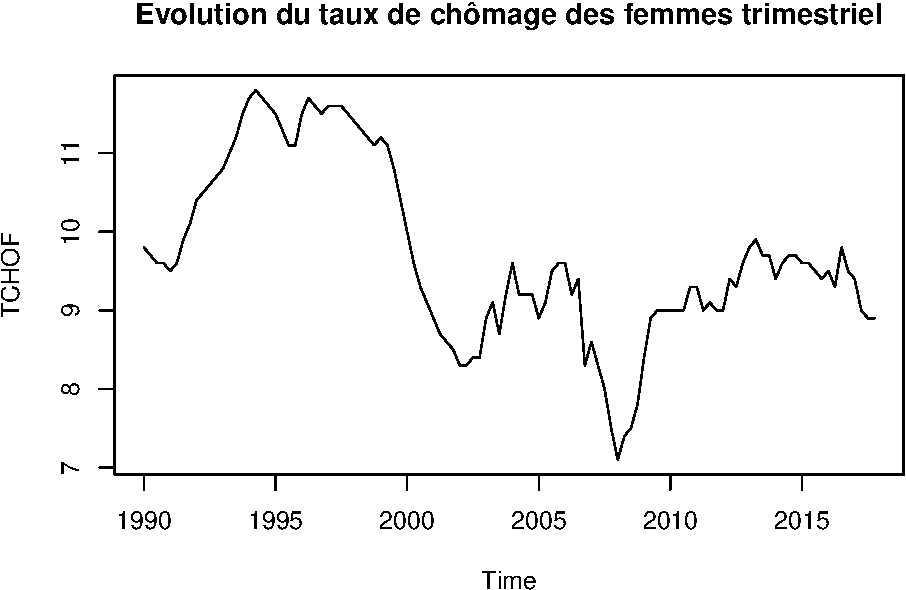
\includegraphics{doc_files/figure-latex/unnamed-chunk-5-1.pdf}

\begin{Shaded}
\begin{Highlighting}[]
  \KeywordTok{par}\NormalTok{(}\DataTypeTok{mfrow=}\KeywordTok{c}\NormalTok{(}\DecValTok{1}\NormalTok{,}\DecValTok{2}\NormalTok{))}
  \KeywordTok{acf}\NormalTok{(TCHOF, }\DataTypeTok{main=}\StringTok{"Auto-corrélation du taux de}
\StringTok{      chômage des femmes trimestriel"}\NormalTok{, }\DataTypeTok{lag.max=}\DecValTok{20}\NormalTok{)}
  \KeywordTok{pacf}\NormalTok{(TCHOF, }\DataTypeTok{main=}\StringTok{"Autocorrélation partielle du}
\StringTok{       taux de chômage des femmes trimestriel"}\NormalTok{, }\DataTypeTok{lag.max=}\DecValTok{20}\NormalTok{)}
\end{Highlighting}
\end{Shaded}

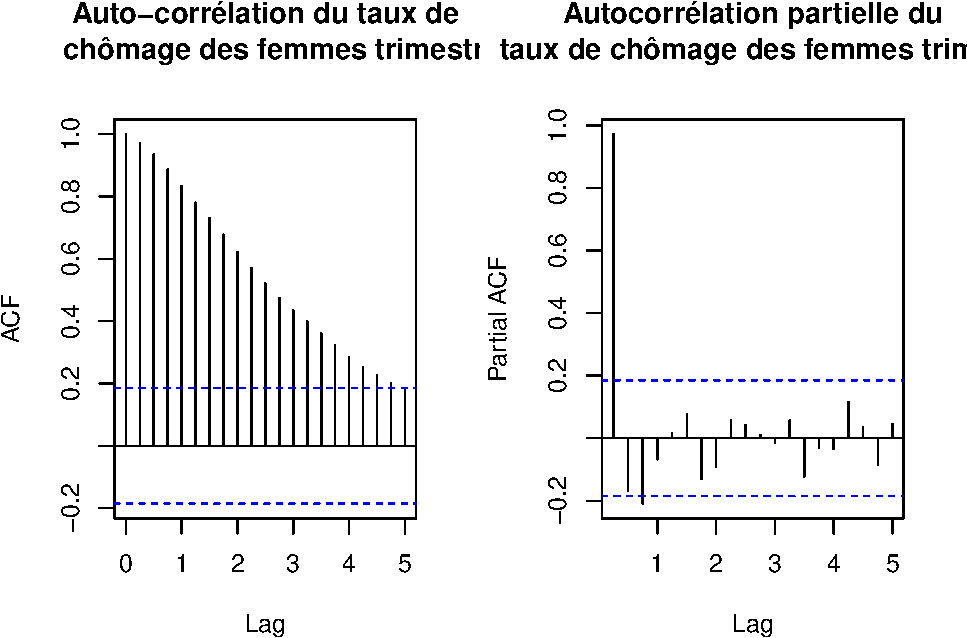
\includegraphics{doc_files/figure-latex/unnamed-chunk-5-2.pdf}

\begin{Shaded}
\begin{Highlighting}[]
  \KeywordTok{par}\NormalTok{(}\DataTypeTok{mfrow=}\KeywordTok{c}\NormalTok{(}\DecValTok{1}\NormalTok{,}\DecValTok{1}\NormalTok{))}
  \KeywordTok{kpss.test}\NormalTok{(TCHOF)}
\end{Highlighting}
\end{Shaded}

\begin{verbatim}
## Warning in kpss.test(TCHOF): p-value smaller than printed p-value
\end{verbatim}

\begin{verbatim}
## 
##  KPSS Test for Level Stationarity
## 
## data:  TCHOF
## KPSS Level = 1.6407, Truncation lag parameter = 2, p-value = 0.01
\end{verbatim}

Pour cette dernière série qui représente le taux de chômage trimestriel
des femmes, il ne semble pas y avoir de saisonnalité. On remarque
cependant qu'il y a bien une tendance. Le test KPSS nous confirme que la
série n'est pas stationnaire. ** Ou est la tendance et de quel type
est-elle ? **

\subsection{Calcul des corrélations}\label{calcul-des-correlations}

\begin{Shaded}
\begin{Highlighting}[]
\NormalTok{trim <-}\StringTok{ }\KeywordTok{read.csv}\NormalTok{(}\StringTok{"~/PFE_Time_Series/Data/Data_Trim.csv"}\NormalTok{, }\DataTypeTok{sep=}\StringTok{";"}\NormalTok{, }\DataTypeTok{dec=}\StringTok{","}\NormalTok{)}
\KeywordTok{corrplot}\NormalTok{(}\KeywordTok{cor}\NormalTok{(trim[}\DecValTok{1}\NormalTok{:}\DecValTok{109}\NormalTok{,-}\DecValTok{1}\NormalTok{]), }\DataTypeTok{method =} \StringTok{"number"}\NormalTok{, }\DataTypeTok{type=}\StringTok{"lower"}\NormalTok{,}
         \DataTypeTok{p.mat=}\KeywordTok{cor.mtest}\NormalTok{(trim[}\DecValTok{1}\NormalTok{:}\DecValTok{109}\NormalTok{,-}\DecValTok{1}\NormalTok{], }\FloatTok{0.95}\NormalTok{)[[}\DecValTok{1}\NormalTok{]], }\DataTypeTok{insig=}\StringTok{"pch"}\NormalTok{,}
         \DataTypeTok{col=}\KeywordTok{colorRampPalette}\NormalTok{(}\KeywordTok{c}\NormalTok{(}\StringTok{"blue"}\NormalTok{, }\StringTok{"light blue"}\NormalTok{, }\StringTok{"red"}\NormalTok{))(}\DecValTok{50}\NormalTok{), }\DataTypeTok{title =} \StringTok{"}
\StringTok{         Corrélations entre les variables trimestrielles"}\NormalTok{)}
\end{Highlighting}
\end{Shaded}

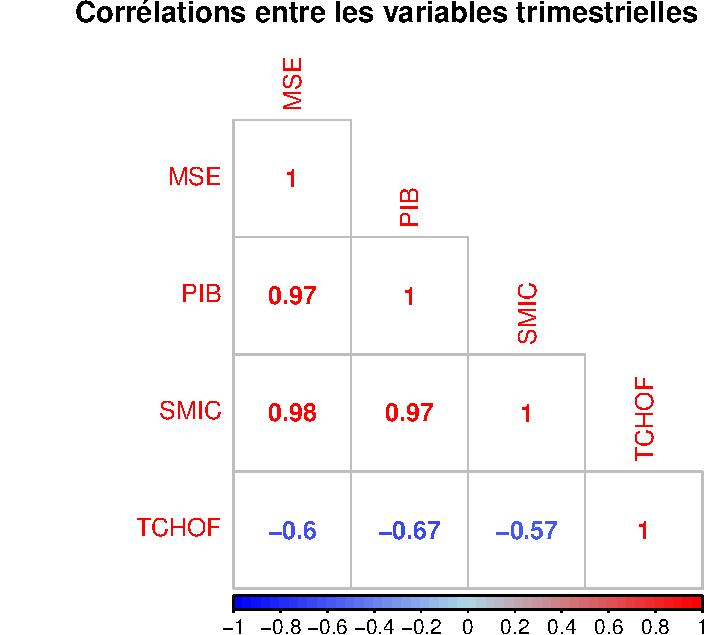
\includegraphics{doc_files/figure-latex/unnamed-chunk-6-1.pdf}

\begin{Shaded}
\begin{Highlighting}[]
\KeywordTok{cor.mtest}\NormalTok{(trim[}\DecValTok{1}\NormalTok{:}\DecValTok{109}\NormalTok{,-}\DecValTok{1}\NormalTok{], }\FloatTok{0.95}\NormalTok{)[[}\DecValTok{1}\NormalTok{]]}
\end{Highlighting}
\end{Shaded}

\begin{verbatim}
##              [,1]         [,2]         [,3]         [,4]
## [1,] 0.000000e+00 3.851955e-69 1.436967e-74 3.321841e-12
## [2,] 3.851955e-69 0.000000e+00 1.898200e-71 2.387179e-15
## [3,] 1.436967e-74 1.898200e-71 0.000000e+00 1.377731e-10
## [4,] 3.321841e-12 2.387179e-15 1.377731e-10 0.000000e+00
\end{verbatim}

On se rend compte que le taux de chômage des femmes est corrélé
négativement avec toutes les autres variables. Le trio de variables PIB,
masse salariale et SMIC sont extrêmement liées entre elles. En regardant
le tableau des p-values associées au test de Student (H0 : La
corrélation entre les deux variables est nulle), on s'aperçoit que
toutes les variables prises deux à deux présentes une corrélation.


\end{document}
